\chapter{Snow}

%%%%%%%%%%%%%%%%%%%%%%%%%%%%%%%%%%%%%%%%%%%%%%%%%%%%%%%%%%%%%%%%
%\section{Introduction}
%%%%%%%%%%%%%%%%%%%%%%%%%%%%%%%%%%%%%%%%%%%%%%%%%%%%%%%%%%%%%%%%

%\begin{figure}[h!]
%\begin{center}
%  \begin{minipage}[c]{.8\textwidth}
%    \centering
%    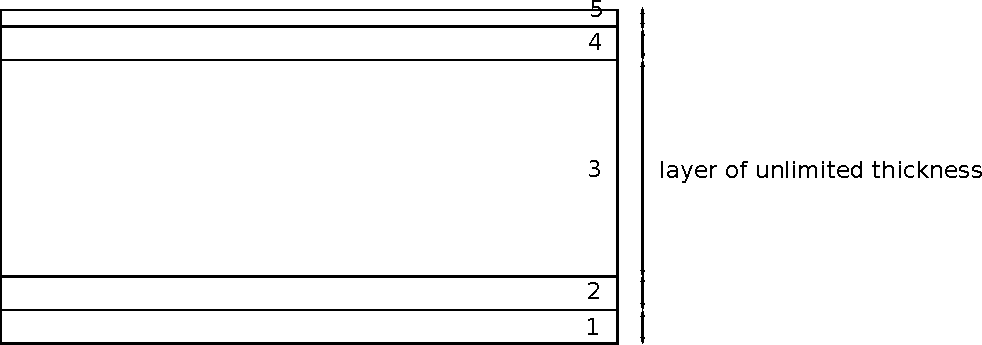
\includegraphics[width=1\textwidth]{./images/pic_snow/snow_layers.pdf}
%  \end{minipage}%
%\end{center}
%\textsl{\caption{Snow stratigraphy}\label{ww}}
%\end{figure}

\section{Input}

\subsection{Parameters}

\begin{center}
\begin{longtable}{|p {4.4 cm}|p {3.7 cm}|p {1. cm}|p{0.8 cm}|p{1.4 cm}|p{0.8 cm}|p{1.3 cm}|}
\hline
\textbf{Keyword} & \textbf{Description} & \textbf{M. U.} & \textbf{range} & \textbf{Default Value} & \textbf{Sca / Vec} & \textbf{Str / Num / Opt} \\ \hline
\endfirsthead
\hline
\multicolumn{7}{| c |}{continued from previous page} \\
\hline
\textbf{Keyword} & \textbf{Description} & \textbf{M. U.} & \textbf{range} & \textbf{Default Value} & \textbf{Sca / Vec} & \textbf{Str / Num / Opt} \\ \hline
\endhead
\hline
\multicolumn{7}{| c |}{{continued on next page}}\\ 
\hline
\endfoot
\endlastfoot
\hline

RoughElemXUnitArea \index{RoughElemXUnitArea} & Number of roughness elements (=vegetation) per unit area - used only for blowing snow subroutines & Number m$^{-2}$ & 0, inf & 0 & sca & num \\ \hline
RoughElemDiam \index{RoughElemDiam} & Diameter of the roughness elements (=vegetation) - used only for blowing snow subroutines & mm & 0, inf & 50 & sca & num \\ \hline
AlphaSnow \index{AlphaSnow} & Alpha (SNTHERM parameter) for the freezing characteristic soil for snow, the bigger, the steeper the curve around 0 degrees & - &  & 1.00E+05 & sca & num \\ \hline
ThresTempRain \index{ThresTempRain} & dew or air temperature above which all precipitation is rain & $^\circ$C &  & 3 & sca & num \\ \hline
ThresTempSnow \index{ThresTempSnow} & dew or air temperature below which all precipitation is snow& $^\circ$C &  & -1 & sca & num \\ \hline
DewTempOrNormTemp \index{DewTempOrNormTemp} & Use dew temperature (1) or air temperature (0) to discriminate between snowfall and rainfall & - & 1 or 0 & 0 & sca & opt \\ \hline
AlbExtParSnow \index{AlbExtParSnow} & albedo extinction parameter (aep): if snow depth $<$ aep, albedo is interpolated between soil and snow & mm &  & 10 & sca & num \\ \hline
FreshSnowReflVis \index{FreshSnowReflVis} & visible band reflectance of fresh snow  & - &  & 0.9 & sca & num \\ \hline
FreshSnowReflNIR \index{FreshSnowReflNIR} & near infrared band reflectance of fresh snow & - &  & 0.65 & sca & num \\ \hline
IrriducibleWatSatSnow \index{IrriducibleWatSatSnow} & Irreducible water saturation. It is the ratio of the capillarity-hold water to ice content in the snow. & - & 0.02 - 0.07 & 0.02 & sca & num \\ \hline
SnowEmissiv \index{SnowEmissiv} & snow long wave emissivity & - &  & 0.98 & sca & num \\ \hline
SnowRoughness \index{SnowRoughness} & Roughness length over snow & mm &  & 0.1 & sca & num \\ \hline
SnowCorrFactor \index{SnowCorrFactor} & correction factor on fresh snow accumulation &  &  & 1 & sca & num \\ \hline
MaxSnowPorosity \index{MaxSnowPorosity} & maximum snow porosity allowed. This parameter prevents excessive snow densification & - &  & 0.7 & sca & num \\ \hline
DrySnowDefRate \index{DrySnowDefRate} & snow compaction (\% per hour) due to destructive metamorphism for snow density$<$ SnowDensityCutoff and dry snow  & - &  & 1 & sca & num \\ \hline
SnowDensityCutoff \index{SnowDensityCutoff} & snow density cutoff to change snow deformation rate & kg m$^{-3}$ &  & 100 & sca & num \\ \hline
WetSnowDefRate \index{WetSnowDefRate} & enhancement factor in presence of wet snow& - &  & 1.5 & sca & num \\ \hline
SnowViscosity \index{SnowViscosity} & snow viscosity coefficient {\bf (kg s m$^{-2}$)} at T=0 C and snow density=0 & N s m$^{-2}$ &  & 1.00E+06 & sca & num \\ \hline
FetchUp \index{FetchUp} & scaling fetch in case snow wind transport in increasing [m] & m &  & 1000 & sca & num \\ \hline
FetchDown \index{FetchDown} & scaling fetch in case snow wind transport in decreasing [m] & m &  & 100 & sca & num \\ \hline
BlowingSnowSoftLayerIceContent \index{BlowingSnowSoftLayerIceContent} & Snow depth (in ice water equivalent), the averaged density of which is used for blowing snow wind thresholds & kg m$^{-2}$ &  & 0 & sca & num \\ \hline
TimeStepBlowingSnow \index{TimeStepBlowingSnow} & Time step [s] at which the Prairie Blowing Snow Model is run & s &  & TimeStep Energy AndWater & sca & num \\ \hline
SnowSMIN \index{SnowSMIN} & minimum slope [degree] to adjust precipitation reduction & degree &  & 30 & sca & num \\ \hline
SnowSMAX \index{SnowSMAX} & maximum slope [degree] to adjust precipitation reduction & degree &  & 80 & sca & num \\ \hline
SnowCURV \index{SnowCURV} & shape parameter for precipitation reduction (if $<$0 the adjustment is not applied) & - &  & -200 & sca & num \\ \hline
MaxWaterEqSnowLayerContent \index{MaxWaterEqSnowLayerContent} & maximum water equivalent admitted in a snow layer & kg m$^{-2}$ &  & 5 & sca & num \\ \hline
MaxSnowLayerNumber \index{MaxSnowLayerNumber} & maximum layers of snow to use (suggested $>$10) &  &  & 10 & sca & num \\ \hline
ThickerSnowLayers \index{ThickerSnowLayers} & Layer numbers that can become thicker than admitted by the threshold given by MaxSnowLayerNumber (from the bottom up). They can be more than one &  &  & Max Snow Layer Number/2 & vec & num \\ \hline
BlowingSnow \index{BlowingSnow} & Activate blowing snow module (yes=1, no=0) & - &  & 0 & sca & opt \\ \hline
PointMaxSWE \index{PointMaxSWE} & Max snow water equivalent that can be reached in the simulation point & kg m$^{-2}$ &  & NA & vec & num \\ \hline
SnowAgingCoeffVis \index{SnowAgingCoeffVis} & reflectance of the new snow in the visible wave length & - &  & 0.2 & sca & num \\ \hline
SnowAgingCoeffNIR \index{SnowAgingCoeffNIR} & reflectance of the new snow in the infrared wave length & - &  & 0.5 & sca & num \\ \hline
\caption{Keywords of snow input parameters configurable in geotop.inpts file.}
\label{snow1d_numeric}
\end{longtable}
\end{center}

\begin{center}
\begin{longtable}{|p {3.4 cm}|p {4.7 cm}|p {1. cm}|p{0.8 cm}|p{1.4 cm}|p{0.8 cm}|p{1.3 cm}|}
\hline
\textbf{Keyword} & \textbf{Description} & \textbf{M. U.} & \textbf{range} & \textbf{Default Value} & \textbf{Sca / Vec} & \textbf{Str / Num / Opt} \\ \hline
\endfirsthead
\hline
\multicolumn{7}{| c |}{continued from previous page} \\
\hline
\textbf{Keyword} & \textbf{Description} & \textbf{M. U.} & \textbf{range} & \textbf{Default Value} & \textbf{Sca / Vec} & \textbf{Str / Num / Opt} \\ \hline
\endhead
\hline
\multicolumn{7}{| c |}{{continued on next page}}\\ 
\hline
\endfoot
\endlastfoot
\hline
ThresSnowSoilRough \index{ThresSnowSoilRough} & Threshold on snow depth to change roughness to snow roughness values with d0 set at 0, for bare soil fraction & mm & 0, 1000 & 10 & vec & num \\ \hline
ThresSnowVegUp \index{ThresSnowVegUp} & Threshold on snow depth above which the roughness is snow roughness, for vegetation fraction & mm & 0, 20000 & 1000 & vec & num \\ \hline
ThresSnowVegDown \index{ThresSnowVegDown} & Threshold on snow depth below which the roughness is vegetation roughness, for vegetation fraction & mm & 0, 20000 & 1000 & vec & num \\ \hline
\caption{Keywords of snow characteristics that may be set in geotop.inpts. Each parameter may be given in input as a vector, each component representing the value corresponding to the LandCoverMapFile value identified by the vector index}
\label{snow_LC_vector}
\end{longtable}
\end{center}


\section{Output}


\subsection{Point output}

\subsubsection{Files}

\begin{center}
\begin{longtable}{|p {3.3 cm}|p {11 cm}|p {2 cm}|p {1 cm}|}
\hline
\textbf{Keyword} & \textbf{Description}  \\ \hline
\endfirsthead
\hline
\multicolumn{4}{| c |}{continued from previous page} \\
\hline
\textbf{Keyword} & \textbf{Description}   \\ \hline
\endhead
\hline
\multicolumn{4}{| c |}{{continued on next page}}\\ 
\hline
\endfoot
\endlastfoot
\hline
SnowProfileFile \index{SnowProfileFile} & name of the output file providing the snow instantaneous values at various depths  \\ \hline
SnowProfileFileWriteEnd \index{SnowProfileFileWriteEnd} & name of the output file providing the snow instantaneous values at various depths written just once at the end  \\ \hline
SnowCoveredAreaFile \index{SnowCoveredAreaFile} & Name of the output file containing the percentage of the area covered by snow \\ \hline
PointOutputFile \index{PointOutputFile} & name of the file providing the properties for the simulation point \\ \hline
PointOutputFileWriteEnd \index{PointOutputFileWriteEnd} & name of the output file providing the Point values written just once at the end \\ \hline
\caption{Keywords of file related to snow / glacier}
\label{snowkeywords_file}
\end{longtable}
\end{center}


\subsubsection{Headers}

\begin{center}
\begin{longtable}{|p {4.3 cm}|p {6.6 cm}|p {2 cm}|p {1 cm}|}
\hline
\textbf{Keyword} & \textbf{Description} & \textbf{Associated file}  \\ \hline
\endfirsthead
\hline
\multicolumn{4}{| c |}{continued from previous page} \\
\hline
\textbf{Keyword} & \textbf{Description} & \textbf{Associated file}  \\ \hline
\endhead
\hline
\multicolumn{4}{| c |}{{continued on next page}}\\ 
\hline
\endfoot
\endlastfoot
\hline
HeaderDateSnow \index{HeaderDateSnow} & column name in the file SnowProfileFile for the variable Date & SnowProfileFile  \\ \hline
HeaderJulianDayFromYear0Snow \index{HeaderJulianDayFromYear0Snow} & column name in the file SnowProfileFile for the variable Julian Day from 0 & SnowProfileFile  \\ \hline
HeaderTimeFromStartSnow \index{HeaderTimeFromStartSnow} & column name in the file SnowProfileFile for the variable Time from start & SnowProfileFile  \\ \hline
HeaderPeriodSnow \index{HeaderPeriodSnow} & column name in the file SnowProfileFile for the variable Simulation period & SnowProfileFile  \\ \hline
HeaderRunSnow \index{HeaderRunSnow} & column name in the file SnowProfileFile for the variable Run & SnowProfileFile  \\ \hline
HeaderIDPointSnow \index{HeaderIDPointSnow} & column name in the file SnowProfileFile for the variable IDPoint & SnowProfileFile  \\ \hline
HeaderTempSnow \index{HeaderTempSnow} & column name in the file SnowProfileFile for the variable temperature & SnowProfileFile  \\ \hline
HeaderIceContentSnow \index{HeaderIceContentSnow} & column name in the file SnowProfileFile for the variable ice content & SnowProfileFile  \\ \hline
HeaderWatContentSnow \index{HeaderWatContentSnow} & column name in the file SnowProfileFile for the variable liquid content & SnowProfileFile  \\ \hline
HeaderDepthSnow \index{HeaderDepthSnow} & column name in the file SnowProfileFile for the variable Depth & SnowProfileFile  \\ \hline
\caption{Keywords of the personalized header for the file SnowProfileFile}
\label{snowheader_data}
\end{longtable}
\end{center}


\begin{center}
\begin{longtable}{|p {3.9 cm}|p {7 cm}|p {2 cm}|p {1 cm}|}
\hline
\textbf{Keyword} & \textbf{Description} & \textbf{Associated file}  \\ \hline
\endfirsthead
\hline
\multicolumn{4}{| c |}{continued from previous page} \\
\hline
\textbf{Keyword} & \textbf{Description} & \textbf{Associated file}  \\ \hline
\endhead
\hline
\multicolumn{4}{| c |}{{continued on next page}}\\ 
\hline
\endfoot
\endlastfoot
\hline
HeaderPsnowNetPoint \index{HeaderPsnowNetPoint} & column name in the file PointOutputFile for the variable PsnowNetPoint & PointOutputFile  \\ \hline
HeaderSnowDepthPoint \index{HeaderSnowDepthPoint} & column name in the file PointOutputFile for the variable SnowDepthPoint & PointOutputFile  \\ \hline
HeaderSWEPoint \index{HeaderSWEPoint} & column name in the file PointOutputFile for the variable SWEPoint & PointOutputFile  \\ \hline
HeaderSnowDensityPoint \index{HeaderSnowDensityPoint} & column name in the file PointOutputFile for the variable SnowDensityPoint & PointOutputFile  \\ \hline
HeaderSnowTempPoint \index{HeaderSnowTempPoint} & column name in the file PointOutputFile for the variable SnowTempPoint & PointOutputFile  \\ \hline
HeaderSnowMeltedPoint \index{HeaderSnowMeltedPoint} & column name in the file PointOutputFile for the variable SnowMeltedPoint & PointOutputFile  \\ \hline
HeaderSnowSublPoint \index{HeaderSnowSublPoint} & column name in the file PointOutputFile for the variable SnowSublPoint & PointOutputFile  \\ \hline
HeaderSWEBlownPoint \index{HeaderSWEBlownPoint} & column name in the file PointOutputFile for the variable SWEBlownPoint & PointOutputFile  \\ \hline
HeaderSWESublBlownPoint \index{HeaderSWESublBlownPoint} & column name in the file PointOutputFile for the variable SWESublBlownPoint & PointOutputFile  \\ \hline
\caption{Keywords of the personalized header for the file PointOutputFile}
\label{snowpoint_data}
\end{longtable}
\end{center}


\subsubsection{Parameters}

\begin{center}
\begin{longtable}{|p {3.4 cm}|p {4.7 cm}|p {1. cm}|p{0.8 cm}|p{1.4 cm}|p{0.8 cm}|p{1.3 cm}|}
\hline
\textbf{Keyword} & \textbf{Description} & \textbf{M. U.} & \textbf{range} & \textbf{Default Value} & \textbf{Sca / Vec} & \textbf{Str / Num / Opt} \\ \hline
\endfirsthead
\hline
\multicolumn{7}{| c |}{continued from previous page} \\
\hline
\textbf{Keyword} & \textbf{Description} & \textbf{M. U.} & \textbf{range} & \textbf{Default Value} & \textbf{Sca / Vec} & \textbf{Str / Num / Opt} \\ \hline
\endhead
\hline
\multicolumn{7}{| c |}{{continued on next page}}\\ 
\hline
\endfoot
\endlastfoot
\hline
DefaultSnow \index{DefaultSnow} & 0: use personal setting, 1:use default & - & 0, 1 & 1 & sca & opt \\ \hline
SnowPlotDepths \index{SnowPlotDepths} & depths of the glacier where one wants to write the results & - &  & NA & vec & num \\ \hline
DateSnow \index{DateSnow} & column number in which one would like to visualize the Date12 [DDMMYYYYhhmm]    	 & - &  & -1 & sca & num \\ \hline
JulianDayFromYear0Snow \index{JulianDayFromYear0Snow} & column number in which one would like to visualize the JulianDayFromYear0[days]   	 & - &  & -1 & sca & num \\ \hline
TimeFromStartSnow \index{TimeFromStartSnow} & column in which one would like to visualize the TimeFromStart[days]     & - &  & -1 & sca & num \\ \hline
PeriodSnow \index{PeriodSnow} & Column number to write the period number & - &  & -1 & sca & num \\ \hline
RunSnow \index{RunSnow} & Column number to write the run number & - &  & -1 & sca & num \\ \hline
IDPointSnow \index{IDPointSnow} & column number in which one would like to visualize the IDpoint  & - &  & -1 & sca & num \\ \hline
WaterEquivalentSnow \index{WaterEquivalentSnow} & column number in which one would like the water equivalent of the snow & - &  & -1 & sca & num \\ \hline
DepthSnow \index{DepthSnow} & column number in which one would like to visualize the depth of the snow & - &  & -1 & sca & num \\ \hline
DensitySnow \index{DensitySnow} & column number in which one would like to visualize the density of the snow & - &  & -1 & sca & num \\ \hline
TempSnow \index{TempSnow} & column number in which one would like to visualize the temperature of the snow  & - &  & -1 & sca & num \\ \hline
IceContentSnow \index{IceContentSnow} & column number in which one would like to visualize the ice content of the snow  & - &  & -1 & sca & num \\ \hline
WatContentSnow \index{WatContentSnow} & column number in which one would like to visualize the water content of the snow  & - &  & -1 & sca & num \\ \hline
\caption{Keywords defining the column number where printing the desired variable in the SnowProfileFile}
\label{snowcolumn_numeric}
\end{longtable}
\end{center}


\begin{center}
\begin{longtable}{|p {3.2 cm}|p {5.3 cm}|p {1 cm}|p{1. cm}|p{1.1 cm}|p{1. cm}|p{1 cm}|}
\hline
\textbf{Keyword} & \textbf{Description} & \textbf{M. U.} & \textbf{range} & \textbf{Default Value} & \textbf{Sca / Vec} & \textbf{Log / Num} \\ \hline
\endfirsthead
\hline
\multicolumn{7}{| c |}{continued from previous page} \\
\hline
\textbf{Keyword} & \textbf{Description} & \textbf{M. U.} & \textbf{range} & \textbf{Default Value} & \textbf{Sca / Vec} & \textbf{Log / Num} \\ \hline
\endhead
\hline
\multicolumn{7}{| c |}{{continued on next page}}\\ 
\hline
\endfoot
\endlastfoot
\hline
DefaultPoint \index{DefaultPoint} & 0: use personal setting, 1:use default & - & 0, 1 & 1 & sca & opt \\ \hline
DtPlotPoint \index{DtPlotPoint} & Plotting Time step (in hour) of the output for specified pixels (0 means the it is not plotted) & h & 0, inf & 0 & vec & num \\ \hline
DatePoint \index{DatePoint} & column number in which one would like to visualize the Date12[DDMMYYYY hhmm]    	 & - & 1, 76 & -1 & sca & num \\ \hline
JulianDayFromYear0Point \index{JulianDayFromYear0Point} & column number in which one would like to visualize the JulianDayFromYear0[days]   	 & - & 1, 76 & -1 & sca & num \\ \hline
TimeFromStartPoint \index{TimeFromStartPoint} & column number in which one would like to visualize the TimeFromStart[days]  & - & 1, 76 & -1 & sca & num \\ \hline
PeriodPoint \index{PeriodPoint} & column number in which one would like to visualize the Simulation\_Period & - & 1, 76 & -1 & sca & num \\ \hline
RunPoint \index{RunPoint} & column number in which one would like to visualize the Run	 & - & 1, 76 & -1 & sca & num \\ \hline
IDPointPoint \index{IDPointPoint} & column number in which one would like to visualize the IDpoint  & - & 1, 76 & -1 & sca & num \\ \hline
SnowDepthPoint \index{SnowDepthPoint} & column number in which one would like to visualize the snow\_depth[mm]  & - & 1, 76 & -1 & sca & num \\ \hline
SWEPoint \index{SWEPoint} & column number in which one would like to visualize the snow\_water\_equivalent [mm]  & - & 1, 76 & -1 & sca & num \\ \hline
SnowDensityPoint \index{SnowDensityPoint} & column number in which one would like to visualize the snow\_density[kg/$^{3}$]  & - & 1, 76 & -1 & sca & num \\ \hline
SnowTempPoint \index{SnowTempPoint} & column number in which one would like to visualize the snow\_temperature[\textcelsius]  & - & 1, 76 & -1 & sca & num \\ \hline
SnowMeltedPoint \index{SnowMeltedPoint} & column number in which one would like to visualize the snow\_melted[mm]  & - & 1, 76 & -1 & sca & num \\ \hline
SnowSublPoint \index{SnowSublPoint} & column number in which one would like to visualize the snow\_subl[mm]  & - & 1, 76 & -1 & sca & num \\ \hline
SWEBlownPoint \index{SWEBlownPoint} & column number in which one would like to visualize the snow\_blown\_away[mm]  & - & 1, 76 & -1 & sca & num \\ \hline
SWESublBlownPoint \index{SWESublBlownPoint} & column number in which one would like to visualize the snow\_subl\_while\_blown [mm] & - & 1, 76 & -1 & sca & num \\ \hline
\caption{Keywords defining the column number where printing the desired variable in the PointOutputFile}
\label{snowcolumnpoint_numeric}
\end{longtable}
\end{center}


\subsection{Map Output}

\subsubsection{Parameters}

\begin{center}
\begin{longtable}{|p {3.4 cm}|p {4.7 cm}|p {1. cm}|p{0.8 cm}|p{1.4 cm}|p{0.8 cm}|p{1.3 cm}|}
\hline
\textbf{Keyword} & \textbf{Description} & \textbf{M. U.} & \textbf{range} & \textbf{Default Value} & \textbf{Sca / Vec} & \textbf{Str / Num / Opt} \\ \hline
\endfirsthead
\hline
\multicolumn{7}{| c |}{continued from previous page} \\
\hline
\textbf{Keyword} & \textbf{Description} & \textbf{M. U.} & \textbf{range} & \textbf{Default Value} & \textbf{Sca / Vec} & \textbf{Str / Num / Opt} \\ \hline
\endhead
\hline
\multicolumn{7}{| c |}{{continued on next page}}\\ 
\hline
\endfoot
\endlastfoot
\hline
DefaultSnow \index{DefaultSnow} & 0: use personal setting, 1:use default & - & 0, 1 & 1 & sca & opt \\ \hline
SnowPlotDepths \index{SnowPlotDepths} & depths of the glacier where one wants to write the results & - &  & NA & vec & num \\ \hline
OutputSnowMaps \index{OutputSnowMaps} & frequency (h) of printing of the results of the snow maps & h &  & 0 & sca & num \\ \hline
\caption{Keywords of frequency for printing snow output maps settable in geotop.inpts}
\label{snowfrequency}
\end{longtable}
\end{center}





